\subsubsection{Reversable Processes}
First we need to talk about reversible processes. A reversible process, broadly speaking, is one that can spontaneously take place in both directions. Let's take a look at an example: say we have two large closed chambers of gas in an isolated system. The only way they can interact is via heat flow.
\begin{figure}[h!]
    \centering
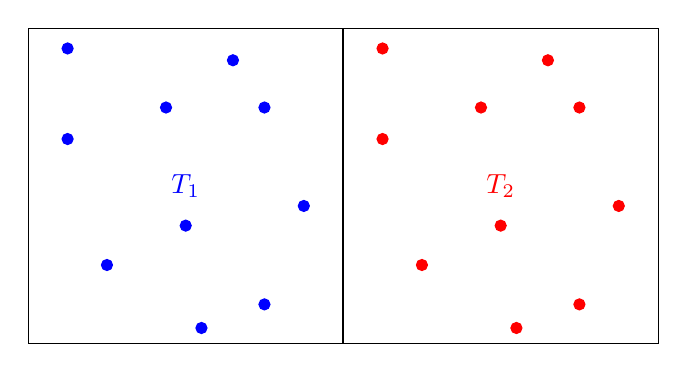
\begin{tikzpicture}
\draw[draw = black] (0,0) rectangle (8,4);
\draw[thick] (4,0) -- (4,4);
\draw[text=blue] (2,2) node {$T_1$};
\draw[text=red] (6,2) node {$T_2$};
\draw[fill=blue, draw=blue] (1,1) circle (2pt);
\draw[fill=blue, draw=blue] (3,0.5) circle (2pt);
\draw[fill=blue, draw=blue] (0.5,2.6) circle (2pt);
\draw[fill=blue, draw=blue] (2.6,3.6) circle (2pt);
\draw[fill=blue, draw=blue] (3.5,1.75) circle (2pt);
\draw[fill=blue, draw=blue] (1.75,3) circle (2pt);
\draw[fill=blue, draw=blue] (2,1.5) circle (2pt);
\draw[fill=blue, draw=blue] (2.2, 0.2) circle (2pt);
\draw[fill=blue, draw=blue] (3,3) circle (2pt);
\draw[fill=blue, draw=blue] (0.5, 3.75) circle (2pt);
\draw[fill=red, draw=red] (5,1) circle (2pt);
\draw[fill=red, draw=red] (7,0.5) circle (2pt);
\draw[fill=red, draw=red] (4.5,2.6) circle (2pt);
\draw[fill=red, draw=red] (6.6,3.6) circle (2pt);
\draw[fill=red, draw=red] (7.5,1.75) circle (2pt);
\draw[fill=red, draw=red] (5.75,3) circle (2pt);
\draw[fill=red, draw=red] (6,1.5) circle (2pt);
\draw[fill=red, draw=red] (6.2, 0.2) circle (2pt);
\draw[fill=red, draw=red] (7,3) circle (2pt);
\draw[fill=red, draw=red] (4.5, 3.75) circle (2pt);
\end{tikzpicture}
    \caption{The wonderful box with two closed sections.}
\end{figure}
\\ If one side is at a higher temperature than the other, then we intuitively know that heat will flow from the hot side to the cool side. But what happens if their temperatures are the same? The short answer is: absolutely nothing. But it's an exciting nothing! Let's dig even deeper. \\
\newline
Say we were to zoom in extremely close on that boundary between the two sides of the box. What would we see? Unsurprisingly, a lot of very small particles hitting a very large wall. However, we know that in order for heat to flow across that barrier, the particles need some way of transferring their energy across the wall. How could they do it? Well, there's two possible ways. The first is radiation, which we'll pretend doesn't exist (it makes our lives much easier, and isn't a terrible assumption). The other is through the wall itself. That is, when a particle collides with the wall, a bit of its kinetic energy goes into the wall, which then gives it up to a particle colliding on the other side.
\newline\newline
Here's the key though: particles on both sides of the wall do this, regardless of the temperature difference. Even if we had the right side of the box at $10^{20}\mathrm{K}$ \footnote{Actually at a temperature this high there would be no box.} and the left side at $100\mathrm{K}$, some particles from the left side of the box would hit the wall and give up some energy to the right side. It's just that particles on the right side of the box are
\begin{enumerate}
    \item Giving up way more energy when they hit the wall.
    \item Hitting the wall far more frequently.
    \item And/or both!
\end{enumerate}
So the \textit{net} transfer of energy is from the right side of the box to the left. In a situation like this, where there is a spontaneous net transfer of energy, we'd say that said process is irreversible. However, if the temperature in the box was the same at both sides, we'd expect no net heat transfer to take place. Therefore, we could conclude that
\begin{itemize}
    \item Both sides give up the same amount of energy per collision on average.
    \item Both sides have the same frequency of collision.
\end{itemize}
This is where the symbol $\delta$ comes in. As the profs may or may not have mentioned in lecture, it means a \textit{very very very} small change. Which, it so happens, is the perfect way to describe the change in energy/temperature each side of the box has when one collision occurs. So we have a very small heat flow, and essentially constant temperature. Furthermore we can see that this tiny flow of heat has an equal chance of happening in both directions, and will. Hence, its reversible!
\newline\newline
So now that we have a better idea of what a reversible process is, we can better understand what entropy is. As a quick reminder, we said above that
\begin{equation*}
    dS=\frac{\delta Q_{rev}}{T}
\end{equation*}
With our newfound knowledge we can say that this says: the change in entropy of a system ($dS$) in a \textit{reversible} heat transfer is \textit{directly} proportional to the amount of heat transferred into the system and \textit{inversely} proportional to the temperature of the system.\footnote{Some of you may wonder if this definition still can be applied when the heat transfer is irreverisible. It can, but the equality is replaced by in inequality $dS > \frac{dQ}{T}$. So if you wanted the most general definition would be $dS \geq \frac{dQ}{T}$.}
\newline\newline
We say above that our tiny reversible processes happen between two systems at the same (constant) temperature. Here's the issue though, and the one that causes us to define all our reversible processes (and entropy) as infinitesimals: no reversible process actually exists on a macroscopic scale.
\newline\newline
As an example of why this is, let's take a look at a process that is theoretically reversible, but isn't actually reversible. Say we have a container of a gas with a piston on one face, but insulated such that it cannot exchange heat (or molecules) with its environment. However, it is connected to a neighbouring infinitely large heat bath, where it can exchange heat with (but not molecules). 
\begin{figure}[h!]
\centering
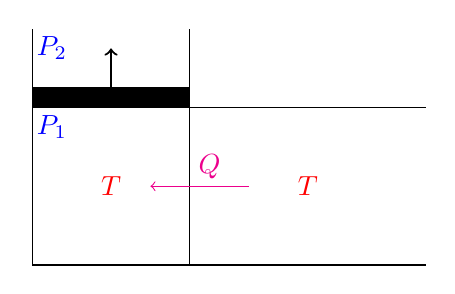
\begin{tikzpicture}
\draw[draw=black] (0,0) rectangle (2,2);
\draw[fill = black] (0,2) rectangle (2,2.25);
\draw (0,2) -- (0,3);
\draw (2,2) -- (2,3);
\draw (2,2) -- (5,2);
\draw (2,0) -- (5,0);
\draw[->, thick] (1, 2.25) -- (1, 2.75);
\draw[text=blue] (0.25,1.75) node {$P_1$};
\draw[text=blue] (0.25, 2.75) node {$P_2$};
\draw[text=red] (1,1) node {$T$};
\draw[text=red] (3.5,1) node {$T$};
\draw[magenta, ->] (2.75,1) -- (1.5,1);
\draw[text=magenta] (2.25, 1.25) node {$Q$};
\end{tikzpicture}
\caption{Piston with infinite heat bath to the right.}
\end{figure}
In this situation, we have that $P_{1}>P_{2}$, so the piston will undergo an expansion. Since the heat bath beside it will keep it at the same temperature, the expansion will be isothermal. So since the temperature of the two sides of the piston/heat bath barrier is constant and equal, the heat transfer across it reversible right? Well, not quite. And it has to do with the idea that a perfectly isothermal process doesn't exist either.
\newline\newline
To figure out why, let's break down what happens step by step. Initially, both the gas and the heat bath are at the same temperature, so no net heat flow between them. However, the pressure inside the piston is greater than the pressure outside. So the piston expands. When it does this, it does work on the environment, and loses energy. This in turn causes its temperature to fall. Its temperature dropping causes heat to flow spontaneously across from the heat bath, until the gas returns to its original temperature. Rinse, repeat until the internal and external pressures are equal.
\newline\newline
So we can see that during an isothermal process, the temperature isn't quite constant. However, if we do this process \textit{very} slowly, the heat flow will manage to restore the temperature so quickly (or to put it another way, heat will flow into the system much faster than the system does work) that the temperature be \textit{almost} constant the whole time. This is what we really mean by an isothermal process. It's also why entropy is defined infinitesimally, since we approximate that each of our tiny expansion steps of the piston happen at constant temperature.
\newline\newline
That being said, imagining an ideal, isothermal process is extremely useful, especially at small time scales. It allows us to derive the following formula for the change in entropy:
\begin{equation}
    \label{eqn:(36)}
    \Delta S=n{c_{v}}\ln{\frac{T_1}{T_0}} + nR\ln{\frac{V_1}{V_0}}
\end{equation}
Here, $n$ is the number of mols of gas, $c_v = \frac{\chi}{2}R$ as we defined earlier (for $\chi$ degrees of freedom and the gas constant $R$), $T_0$ and $T_1$ are the initial and final temperatures, and $V_0$ and $V_1$ are the initial and final volumes. First, the change in entropy depends only on the initial and final states of the system (i.e. the final and initial temperatures and volumes), not the path between those states! So \textbf{entropy is function of state}.
\newline\newline
The second thing you should notice is that entropy of a system is dependent on the volume, an \textit{extensive} quantity. Therefore, \textbf{entropy is an extensive quantity}.

\subsubsection{(Optional) Derivation of the Sackur–Tetrode Equation}
Equation \ref{eqn:(36)} as shown above is actually a version of the Sackur-Tetrode equation, which gives the entropy of a monoatomic ideal gas in full. While the derivation of the full equation is far, far out of the scope of this course\footnote{You may consult Wikipedia if you want to see the full equation}, equation \ref{eqn:(36)} can totally be derived with the things we have learned. This derivation is more for your curiousity than anything, and you do already have all the tools required to derive it (so if you're keen, give it a shot!). We start from the definition of entropy (for a reversible heat transfer):
\begin{align*}
    dS = \frac{dQ}{T}
\end{align*}
Now, we consider the first law of Thermodynamics:
\[
    dE = dQ+dW
\]
So let us substitute $dQ = dE-dW$ to obtain:
\[ dS = \frac{dE-dW}{T} = \frac{dE}{T}-\frac{dW}{T}
\]
We apply the (at this point, well-acquainted) formula for change in energy:
\[dE = nc_vdT \]
And we hence obtain:
\[ dS = \frac{nc_vdT}{T} - \frac{dW}{T} \]
We may now use the ideal gas law:
\[T = \frac{PV}{nR} \]
As well as the definition of work:
\[dW = -PdV \]
Substituting these in, we obtain:
\[ dS = \frac{nc_vdT}{T} + \frac{PdV}{\frac{PV}{nR}}\]
Which simplifies to:
\[dS = nc_v\frac{dT}{T} + nR\frac{dV}{V} \]
Now, we integrate from an initial state to a final state (in other words, from a initial entropy/temperature/volume $S_0,T_0,V_0$ to a final entropy/temperature/volume $S_1,T_1,V_1$:
\[\int_{S_0}^{S_1} dS = \int_{T_0}^{T_1}nc_v\frac{dT}{T} + \int_{V_0}^{V_1}nR\frac{dV}{V} \]
Performing the integration, we obtain:
\[ \left.S \right|_{S_0}^{S_1} = nc_v \left. \ln(T) \right|_{T_0}^{T_1} + nR \left. \ln(V) \right|_{V_0}^{V_1} \]
\[ \Delta S = nc_v\ln\left(\frac{T_1}{T_0}\right) + nR \ln\left(\frac{V_1}{V_0}\right) \]
Which is the desired result. 